\documentclass[a4paper,oneside]{book}
\usepackage[pagestyles]{titlesec}
\usepackage{xeCJK}
\usepackage{fontspec}
\usepackage[top=2.0cm,bottom=2.0cm,left=2.0cm,right=2.0cm]{geometry}
\usepackage{xcolor}
\usepackage{color}
\usepackage{mdframed}
\usepackage{listings}
\usepackage{caption}
\usepackage{fancybox}
\usepackage{indentfirst}
\usepackage{dirtree}
\usepackage[titles]{tocloft}
\usepackage{hyperref}
%\usepackage[pagestyles]{titlesec}%设置章节标题格式,居中(center)
\setmainfont{Times New Roman}%设置英文主字体
\setCJKmainfont{AR PL UKai TW MBE}%设置中文主字体
\setmonofont[Mapping={}]{SimSun}%设置等宽字体

\renewcommand{\baselinestretch}{1.2}%设置行距,1.2倍行距
\titleformat{\chapter}{\Huge\bfseries}{第\thechapter 章}{1em}{}%command=chapter,format=\centring...,label=第\thechapter...其它忽略
\titlespacing*{\chapter}{0pt}{\baselineskip}{\baselineskip}%设置章下面的空白
\titleformat{\section}{\Large\bfseries}{\thesection}{1em}{}%设置节字体大小,属性

\newcommand{\wordred}[1]{{\color{red}{#1}}}

%页眉与页脚设置
\newpagestyle{main}{
\sethead{\small\S\,\thesection\quad\sectiontitle}{}{$\cdot$~\thepage~$\cdot$}%这里是单页面页眉设置,不能用于双页面
\setfoot{}{}{}\headrule}
\pagestyle{main}

%设置C语言代码框
\lstset{numbers=left,
numberstyle=\footnotesize,
basicstyle=\footnotesize\ttfamily,
keywordstyle=\color{blue!70},
commentstyle=\color{red!0!green!0!blue!100},
frame=shadowbox,
rulesepcolor=\color{red!20!green!20!blue!20},
tabsize=4,%设置tab键空格数
escapeinside=@@%设置逃逸字串,用来显示代码框的中文
}

%设置框类型,单边,红色
\mdfsetup{skipabove=\topskip,skipbelow=\topskip}
\global\mdfdefinestyle{leftredline}{
linecolor=red,
linewidth=3pt,
topline=false,
bottomline=false,
font=\footnotesize,
}

%设置代码目录树
\renewcommand*\DTstylecomment{\rmfamily\textsc}
\renewcommand*\DTstyle{\ttfamily\textcolor{black}}

%目录设置

\definecolor{ubuntured}{RGB}{44,0,30}

\begin{document}
\chapter{UBIFS简介}
无序区块镜像文件系统(Unsorted Block Image File System, UBIFS)是用于固态存储设备上,并与LogFS相互竞争,作为JFFS2的后继文件系统之一。

UBIFS是专门为了解决MTD(Memory Technology Device)设备所遇到的性能瓶颈而设计的。由于Nand Flash容量的暴涨,YAFFS等皆无法操控大的Nand Flash空间。UBIFS通过子系统UBI处理与MTD device之间的动作。与JFFS2一样,UBIFS 建构于MTD device 之上,因而与一般的block device(例如: emmc, sd-card等)不兼容。

\section{UBI子系统}
JFFS2与UBIFS区别是,JFFS2是可以直接操作MTD设备,而UBIFS是工作在UBI卷上。因此对于UBIFS来说其实有三个子系统:
\begin{itemize}
  \item MTD子系统,它提供了访问flash的标准接口,并向上层应用程序提供类似/dev/mtd[0-99]接口
  \item UBI子系统,它为flash提供了损耗均衡与卷管理系统,UBI是MTD的高层次表示,为UBIFS处理flash的坏块管理与损耗均衡等工作
  \item UBIFS文件系统,工作在UBI卷上
\end{itemize}

UBI卷,与分区概念类似,一个分区是一组连续的物理地址的集合,而卷是一组连续的逻辑地址集合,所以卷中的擦除块又称为逻辑擦除块。这个逻辑块可以映射到分区上任一个物理块上。UBI有两种卷类型,可读写的动态卷与只读的静态卷。

UBI卷层(layout volume),卷层是一个特殊的卷,称为内部卷,它里面包含了ubi的卷表信息。卷层包含两个逻辑擦除块,其中一个卷是为了备份另一个卷而存在的。

UBI坏块管理,UBI的存在使得UBIFS不用关注坏块问题。UBI会在flash中预留一部分的冗余块,这些块是用来替换使用过程中出现的坏块。UBI将旧块数据移动到替换块上,然后改变UBI卷中的逻辑块到物理块的映射关系。

UBI冲刷机制,因为ECC的存在,flash少量的bit-flip是不会导致系统出现问题的,但是bit-flip累积到一定数量就会导致系统出现问题。UBI冲刷是针对出现bit-flip的块,把待冲刷块数据搬迁到其它块上,然后对这个块进行擦除操作,以确定它是不是坏块。

UBI损耗均衡,UBI会记录每一个块擦除次数,对于擦除次数过多的块,会把它的数据移到擦除次数少的块,然后改变卷的逻辑块到物理块的映射。


\chapter{MTD驱动分析}
\section{MTD简介}
MTD,Memory Technology Device即内存技术设备,MTD的存在屏蔽了flash驱动实现细节,向上(主要指文件系统)提供统一的API接口。并且MTD只能工作在raw flash上,目前市面上主要有以下几种类型的flash
\begin{itemize}
  \item raw flash,原始flash设备,采用ONFI接口,只有基本的存储功能 。不提供ecc除错,坏块管理,负载均衡等机制,这些都是由host processor提供
  \item clear flash,将ECC机制整合进了flash芯片中的新型flash,采用ONFI接口
  \item emmc,将nand flash与控制芯片封装在一起,提供了ECC除错,坏块管理,负载均衡等机制,采用JEDEC标准 
  \item UFS,通用flash存储器,具备emmc功能,并且可以读写数据同时进行,采用JEDEC标准
\end{itemize}

\section{MTD驱动结构}
MTD向用户空间提供了字符设备节点与块设备节点供用户空间程序直接操作flash设备,向文件系统提供了MTD原始设备层,文件系统不再关心flash驱动具体实现

\begin{figure}[htbp]
\centering
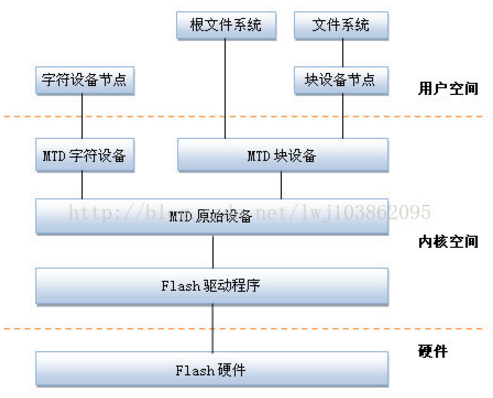
\includegraphics[keepaspectratio,width=0.5\textwidth,height=0.75\textheight]{img/mtd_struct.png}
\end{figure}
在上图中可以发现,MTD原始设备是对NandFlash封装的一层。下面主要分析原始设备层是如何使用NandFlash驱动,以及向上层提供了哪些封装函数

\section{MTD原始设备层}
操作NandFlash主要有三个动作,读/写/擦除。MTD原始设备在read/write/erase函数中会调用nand flash chip驱动的相应操作方法,而文件系统则可以直接使用原始设备层提供的read/write/erase去操作flash。
\clearpage
\subsection{主要数据结构分析}
struct mtd\_info就代表MTD原始设备层,这个结构体的函数是需要驱动开发人员实现的,实现这些函数比较简单,基本都是直接调用nand flash驱动的函数。
\begin{lstlisting}[language=C]
struct mtd_info {
	u_char type; //nor flash or nand flash(mlc/slc/tlc)
	uint32_t flags; //mtd-abi.h中定义它的属性值
	uint64_t size; //mtd设备大小,就是分区大小
	uint32_t erasesize; //block大小
	uint32_t writesize; //最小写单位,对于nandflash就是PageSize(或subPageSize)
	uint32_t writebufsize; //基本未使用,writebufsize可以减少向flash写入次数
	uint32_t oobsize; //OOB字节数,spare space size
	uint32_t oobavail; //可用OOB字节数
	unsigned int erasesize_shift; //默认0
	unsigned int writesize_shift; //默认0
	unsigned int erasesize_mask;  //默认0
	unsigned int writesize_mask;  //默认0
	unsigned int bitflip_threshold; //bitflip数超过这个值,就会报EUCLEAN错误,这个值可以通过sysfs修改
	const char *name; //mtd名字,一般就是分区名cat /proc/mtd读出来的
	int index; //不重要
	struct nand_ecclayout *ecclayout; //ecc在oob中布局,根据硬件得到
	unsigned int ecc_step_size; //一次对多少字节进行校验计算,一般是256或512字节
	unsigned int ecc_strength; //可校准bitflip位数
	int numeraseregions; //不同的erasesize区域数目,通常都是1
	struct mtd_erase_region_info *eraseregions;
	int (*_erase) (struct mtd_info *mtd, struct erase_info *instr); //块擦除函数
	... ...
	int (*_read) (struct mtd_info *mtd, loff_t from, size_t len,
		      size_t *retlen, u_char *buf); //读page函数
	int (*_write) (struct mtd_info *mtd, loff_t to, size_t len,
		       size_t *retlen, const u_char *buf); //写page函数
	int (*_panic_write) (struct mtd_info *mtd, loff_t to, size_t len,
			     size_t *retlen, const u_char *buf);
	int (*_read_oob) (struct mtd_info *mtd, loff_t from,
			  struct mtd_oob_ops *ops); //带oob读函数
	int (*_write_oob) (struct mtd_info *mtd, loff_t to,
			   struct mtd_oob_ops *ops); //带oob写函数
	... ...
	void (*_sync) (struct mtd_info *mtd);
	int (*_lock) (struct mtd_info *mtd, loff_t ofs, uint64_t len); //nandflash支持设备独占访问才能定义
	int (*_unlock) (struct mtd_info *mtd, loff_t ofs, uint64_t len);//nandflash解锁
	int (*_is_locked) (struct mtd_info *mtd, loff_t ofs, uint64_t len);
	int (*_block_isreserved) (struct mtd_info *mtd, loff_t ofs);
	int (*_block_isbad) (struct mtd_info *mtd, loff_t ofs); //坏块判断函数
	int (*_block_markbad) (struct mtd_info *mtd, loff_t ofs); //使用中出现坏块时的标记函数
	int (*_suspend) (struct mtd_info *mtd);
	void (*_resume) (struct mtd_info *mtd);
	int (*_get_device) (struct mtd_info *mtd);
	void (*_put_device) (struct mtd_info *mtd);
	struct backing_dev_info *backing_dev_info;
	struct notifier_block reboot_notifier;
	struct mtd_ecc_stats ecc_stats;
	int subpage_sft;
	void *priv;
	struct module *owner;
	struct device dev;
	int usecount;
};

\end{lstlisting}
\clearpage
struct nand\_chip结构体代表的是flash驱动,它是直接与硬件通信的,因此nand\_chip中的需要用到的函数都是由驱动开发人员实现。nand chip也不必使用MTD自带的struct nand\_chip,驱动开发自己定义,然后自己实现也是可以的,高通自定义的为struct msm\_nand\_chip。
\begin{lstlisting}[language=C]
struct nand_chip {
	void __iomem *IO_ADDR_R; //读写8根IO线的地址
	void __iomem *IO_ADDR_W;
	uint8_t (*read_byte)(struct mtd_info *mtd); //读flash单一字节
	u16 (*read_word)(struct mtd_info *mtd);
	void (*write_byte)(struct mtd_info *mtd, uint8_t byte);
	void (*write_buf)(struct mtd_info *mtd, const uint8_t *buf, int len);
	void (*read_buf)(struct mtd_info *mtd, uint8_t *buf, int len);
	void (*select_chip)(struct mtd_info *mtd, int chip);
	int (*block_bad)(struct mtd_info *mtd, loff_t ofs, int getchip);
	int (*block_markbad)(struct mtd_info *mtd, loff_t ofs);
	void (*cmd_ctrl)(struct mtd_info *mtd, int dat, unsigned int ctrl);
	int (*init_size)(struct mtd_info *mtd, struct nand_chip *this,
			u8 *id_data);
	int (*dev_ready)(struct mtd_info *mtd);
	void (*cmdfunc)(struct mtd_info *mtd, unsigned command, int column,
			int page_addr);
	int(*waitfunc)(struct mtd_info *mtd, struct nand_chip *this);
	int (*erase)(struct mtd_info *mtd, int page);
	int (*scan_bbt)(struct mtd_info *mtd);
	int (*errstat)(struct mtd_info *mtd, struct nand_chip *this, int state,
			int status, int page);
	int (*write_page)(struct mtd_info *mtd, struct nand_chip *chip,
			uint32_t offset, int data_len, const uint8_t *buf,
			int oob_required, int page, int cached, int raw);
	int (*onfi_set_features)(struct mtd_info *mtd, struct nand_chip *chip,
			int feature_addr, uint8_t *subfeature_para);
	int (*onfi_get_features)(struct mtd_info *mtd, struct nand_chip *chip,
			int feature_addr, uint8_t *subfeature_para);
	int (*setup_read_retry)(struct mtd_info *mtd, int retry_mode);
	int chip_delay;
	unsigned int options;
	unsigned int bbt_options;
	int page_shift;
	int phys_erase_shift;
	int bbt_erase_shift;
	int chip_shift;
	int numchips;
	uint64_t chipsize;
	int pagemask;
	int pagebuf;
	unsigned int pagebuf_bitflips;
	int subpagesize;
	uint8_t bits_per_cell;
	uint16_t ecc_strength_ds;
	uint16_t ecc_step_ds;
	int onfi_timing_mode_default;
	int badblockpos;
	int badblockbits;
	int onfi_version;
	int jedec_version;
	union {
		struct nand_onfi_params	onfi_params;
		struct nand_jedec_params jedec_params;
	};
	int read_retries;
	flstate_t state;
	uint8_t *oob_poi;
	struct nand_hw_control *controller;
	struct nand_ecc_ctrl ecc;
	struct nand_buffers *buffers;
	struct nand_hw_control hwcontrol;
	uint8_t *bbt;
	struct nand_bbt_descr *bbt_td;
	struct nand_bbt_descr *bbt_md;
	struct nand_bbt_descr *badblock_pattern;
	void *priv;
};

\end{lstlisting}

























\chapter{UBI子系统分析}

%********************新章开始*******************************%
\chapter{UBI镜像调试与制作}
\section{UBI镜像在ubuntu中调试优点}
编译出来的需要烧录到模块的ubi镜像是可以放在ubuntu下面进行挂载调试,可以直接利用PC操作模块的文件系统,其优点如下:
\begin{itemize}
  \item PC机的高性能有助于开发人员快速搜索分析ubifs镜像中的可执行文件,配置文件,脚本文件等
  \item 对于配置文件与脚本文件可以直接修改,重新打包下载到模块中
  \item 可以直接确定ubi镜像是否包含修改后代码的编译结果
\end{itemize}
UBI镜像在ubuntu上的调试与制作只需要进行如下工具安装:

\begin{mdframed}[backgroundcolor=lightgray,hidealllines=true]
\begin{verbatim}

darren@darren:~$sudo apt-get install mtd-untils

\end{verbatim}
\end{mdframed}

\section{ubi文件结构主要参数分析}
在挂载ubi文件系统之前,首先要清楚它的几个参数,PEB( Physical Erase Block ),LEB( Logical Erase Blcok ),Page Size,下面是分析linux rootfs的过程:
\begin{mdframed}[backgroundcolor=lightgray,hidealllines=true]
\begin{verbatim}

darren@darren:~$ hexdump -C mdm-perf-recovery-image-mdm9607-perf.ubi | grep "UBI#"
00000000  55 42 49 23 01 00 00 00  00 00 00 00 00 00 00 00  |UBI#............|
00040000  55 42 49 23 01 00 00 00  00 00 00 00 00 00 00 00  |UBI#............|
00080000  55 42 49 23 01 00 00 00  00 00 00 00 00 00 00 00  |UBI#............|
000c0000  55 42 49 23 01 00 00 00  00 00 00 00 00 00 00 00  |UBI#............|
00100000  55 42 49 23 01 00 00 00  00 00 00 00 00 00 00 00  |UBI#............|
00140000  55 42 49 23 01 00 00 00  00 00 00 00 00 00 00 00  |UBI#............|
00180000  55 42 49 23 01 00 00 00  00 00 00 00 00 00 00 00  |UBI#............|

\end{verbatim}
\end{mdframed}

"UBI\#"是struct ubi\_ec\_hdr的魔数,这里的魔数可以简单的理解为标识一个PEB的开始,这里的魔数值可在内核代码中查到,由上可得\wordred{PEB SIZE = 0x0004,0000 - 0x0000,0000 = 256KB}
\begin{mdframed}[backgroundcolor=lightgray,hidealllines=true]
\begin{verbatim}

darren@darren:~$ hexdump -C mdm-perf-recovery-image-mdm9607-perf.ubi | grep "UBI!"
00001000  55 42 49 21 01 01 00 05  7f ff ef ff 00 00 00 00  |UBI!............|
00041000  55 42 49 21 01 01 00 05  7f ff ef ff 00 00 00 01  |UBI!............|
00081000  55 42 49 21 01 01 00 00  00 00 00 00 00 00 00 00  |UBI!............|
000c1000  55 42 49 21 01 01 00 00  00 00 00 00 00 00 00 01  |UBI!............|
00101000  55 42 49 21 01 01 00 00  00 00 00 00 00 00 00 02  |UBI!............|
00141000  55 42 49 21 01 01 00 00  00 00 00 00 00 00 00 03  |UBI!............|
00181000  55 42 49 21 01 01 00 00  00 00 00 00 00 00 00 04  |UBI!............|

\end{verbatim}
\end{mdframed}

"UBI!"是struct ubi\_vid\_hdr的魔数,ubi\_vid\_hdr是标识一个已经分配到ubi卷中的PEB,它与struct ubi\_ec\_hdr各占PEB的前两页中的一页,\wordred{Page SIZE = 0x0000,1000 - 0x0000,0000 = 4KB}

LEB的大小是PEB减去所有头部后剩下的空间,PEB的所头部就是struct ubi\_vid\_hdr与struct ubi\_ec\_hdr,因此,\wordred{LEB SIZE = PEB SIZE - 2*Page SIZE = 248KB}

\section{虚拟MTD设备并挂载ubifs}
正常情况下,我们的ubi镜像是根据flash的参数来确定PEB,LEB,Page SIZE的,但是现在ubi已经做好,所以我们需要根据ubi参数反向推导出flash参数,flash采用的是MTD驱动架构。目前市场上大部份flash都是遵守ONFI( Open Nand Flash Interface )标准,这个标准是由英特尔,闪迪,索尼等多家flash厂商联合制定的,在这份标准中规定,寄存器90H是flash的ID寄存器,这个寄存器包含5个字节的数据。而90H的第四个字节决定了flash的Page SIZE,block SIZE等参数

\begin{figure}[htbp]
\centering
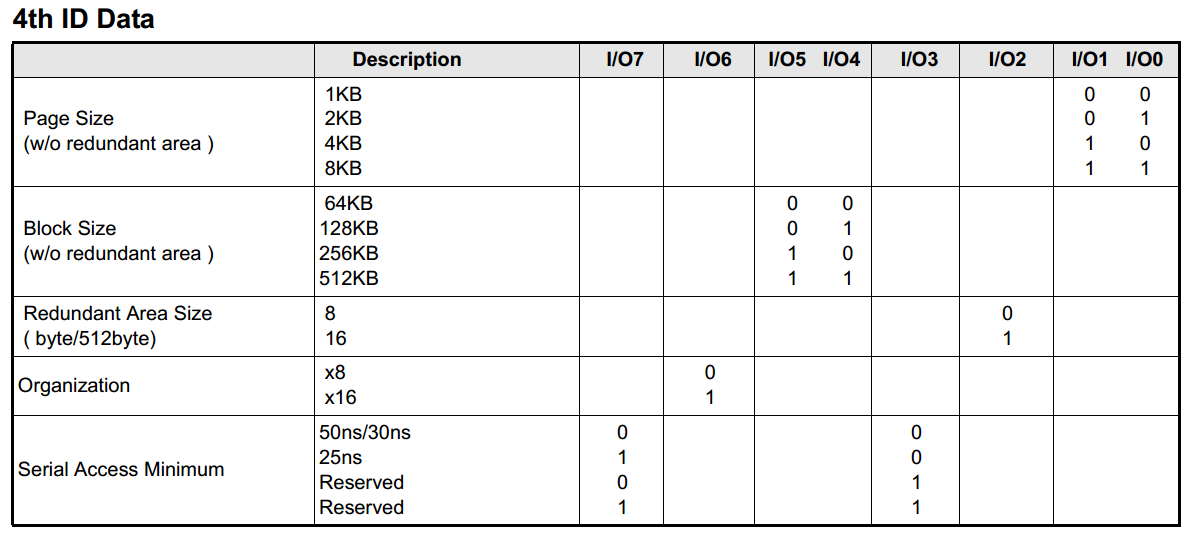
\includegraphics[keepaspectratio,width=\textwidth,height=0.75\textheight]{img/20170517170203.png}
\end{figure}
根据上图获取的信息,就可以使用modprobe nandsim在ubuntu上模拟一个MTD设备了,nandsim的fourth\_id\_byte是我们关注的参数,其它参数可以从ONFI文档中获取
\begin{mdframed}[backgroundcolor=lightgray,hidealllines=true]
\begin{verbatim}

darren@darren:~$ sudo modprobe nandsim first_id_byte=0xec second_id_byte=0xd3
third_id_byte=0x10 fourth_id_byte=0xa6
darren@darren:~$ mtdinfo /dev/mtd0
mtd0
Name:                           NAND simulator partition 0
Type:                           nand
Eraseblock size:                262144 bytes, 256.0 KiB
Amount of eraseblocks:          4096 (1073741824 bytes, 1024.0 MiB)
Minimum input/output unit size: 4096 bytes
Sub-page size:                  1024 bytes
OOB size:                       128 bytes
Character device major/minor:   90:0
Bad blocks are allowed:         true
Device is writable:             true

\end{verbatim}
\end{mdframed}
安装ubi模块,并利用uevent生成/dev/ubi\_ctrl设备节点
\begin{mdframed}[backgroundcolor=lightgray,hidealllines=true]
\begin{verbatim}

darren@darren:~$ sudo modprobe ubi
darren@darren:~$ sudo su
root@darren:~$ echo "add" > /sys/devices/virtual/misc/ubi_ctrl/uevent

\end{verbatim}
\end{mdframed}
将ubi镜像刷入虚拟MTD分区中
\begin{mdframed}[backgroundcolor=lightgray,hidealllines=true]
\begin{verbatim}

darren@darren:~$ sudo ubiformat /dev/mtd0 -f mdm9607-perf-sysfs.ubi -O 4096

\end{verbatim}
\end{mdframed}
注意:这里加-O 4096的目的是让struct ubi\_vid\_hdr所处的位置是一个PEB开始的4096偏移处,如果不这样做,那么struct ubi\_vid\_hdr会处于一个Sub-page size大小的偏移处。如果Sub-page size就是4096,那么就没必要加-O选项了。
\vspace{12 pt}

\noindent 建立MTD设备与ubi联系,并挂载ubi文件系统
\begin{mdframed}[backgroundcolor=lightgray,hidealllines=true]
\begin{verbatim}

darren@darren:~$ sudo ubiattach -m 0 -O 4096
UBI device number 0, total 4096 LEBs (1040187392 bytes, 992.0 MiB), available 0 LEBs (0 bytes), 
LEB size 253952 bytes (248.0 KiB)
darren@darren:~$ mkdir rootfs usrfs
darren@darren:~$ sudo mount -t ubifs /dev/ubi0_0 rootfs/
darren@darren:~$ sudo mount -t ubifs /dev/ubi0_1 usrfs/

\end{verbatim}
\end{mdframed}
至此,ubifs已经成功挂载到ubuntu上了,可以对ubi镜像进行内容搜索,文件修改等操作

\section{反向制作ubi镜像}
制作ubi镜像主要用到两个工具,mkfs.ubifs与ubinize。mkfs.ubifs产生的是ubifs,其中是没有卷标信息的,是不能直接烧写到flash上,但可以通过bootloader中的ubi write函数进行烧写。ubinize产生的是完整的ubi镜像,可以直接烧到flash上进行挂载操作。
\begin{mdframed}[backgroundcolor=lightgray,hidealllines=true]
\begin{verbatim}

darren@darren:~$ mkfs.ubifs -m 4096 -e 253952  -c 2146 -r rootfs/ -F -o rootfs.ubifs
darren@darren:~$ mkfs.ubifs -m 4096 -e 253952  -c 2146 -r usrfs/ -F -o usrfs.ubifs
darren@darren:~$ mkfs.ubifs --help
Usage: mkfs.ubifs [OPTIONS] target
Make a UBIFS file system image from an existing directory tree
Options:
-r, -d, --root=DIR      build file system from directory DIR
-m, --min-io-size=SIZE  minimum I/O unit size(page size)
-e, --leb-size=SIZE     logical erase block size(LEB大小)
-c, --max-leb-cnt=COUNT maximum logical erase block count(只要不比最大容量小就可以)

\end{verbatim}
\end{mdframed}
ubi文件系统做好后,就可以利用ubinize来进行ubi镜像制作。这里要注意,有些ubi镜像包含多个卷,那么每个\wordred{需要内容的卷}都是需要用mkfs.ubifs进行文件系统制作。不需要内容的卷可以直接使用ubinize创建新卷(例如下边的cache卷就是不需要内容的卷)。使用ubinize时,需要一个配置文件,这里写了一个配置文件ubinize.ini
\begin{mdframed}[backgroundcolor=lightgray,hidealllines=true]
\begin{verbatim}

darren@darren:~$ cat ubinize.ini
[sysfs_volume]
mode=ubi
image=rootfs.ubifs
vol_id=0
vol_type=dynamic
vol_name=rootfs
vol_size=63MiB
[usrfs_volume]
mode=ubi
image=usrfs.ubifs
vol_id=1
vol_type=dynamic
vol_name=usrfs
vol_flags = autoresize
[cache_volume]
mode=ubi
vol_id=2
vol_type=dynamic
vol_name=cachefs
vol_size=55MiB
darren@darren:~$ sudo ubinize -o system.ubi -p 256KiB -m 4096 -s 4096 ubinize.ini
darren@darren:~$ ubinize --help
ubinize version 1.5.0 - a tool to generate UBI images. An UBI image may contain one 
or more UBI volumes which have to be defined in the input configuration ini-file
Options:
-o, --output=<file name>    output file name
-p, --peb-size=<bytes>      size of the physical eraseblock of the flash(Kib,Mib可以使用)
-m, --min-io-size=<bytes>   minimum input/output unit size of the flash in byte
-s, --sub-page-size=<bytes> minimum input/output unit used for UBI headers(ubi头部偏移)

\end{verbatim}
\end{mdframed}
至此反向制作的镜像就完成了,system.ubi可以使用前面的方法挂载到ubuntu中使用,也可以直接烧写到模块中进行验证。
\section{删除虚拟MTD设备}
虚拟的MTD设备就是一个nandsim模块,卸载这个模块就行了,在卸载之前,需要把所有挂载在它上面的ubi文件系统umount掉,然后把它与ubi的连接断开
\begin{mdframed}[backgroundcolor=lightgray,hidealllines=true]
\begin{verbatim}

darren@darren:~$ sudo umount rootfs/ usrfs/
darren@darren:~$ sudo ubidetach -m 0
darren@darren:~$ sudo rmmod nandsim

\end{verbatim}
\end{mdframed}
这里,扫尾工作也已经完成。上述过程虽然比较繁琐,但是可以利用脚本来操作,使挂载,制作,卸载等一键完成


\end{document}
